\title{ A Traveling Salesman Solution For The Capitals of All African Nations }
\author{
Brian Gianforcaro \\
Department of Computer Science\\
Rochester Institute of Technology\\
}

\date{\today}

\documentclass[12pt]{article}

\usepackage{graphicx}
\usepackage{multicol}
\usepackage{mdwlist}
\usepackage{amssymb,amsmath}
\usepackage{cite}
\usepackage[bookmarks=false,colorlinks=true,linkcolor={blue},pdfstartview={XYZ null null 1.22}]{hyperref}
\usepackage{url}
\usepackage[T1]{fontenc}
%\usepackage{gfsartemisia-euler}


\begin{document}
\maketitle

\begin{abstract}
  A Traveling Salesman Problem is the task of finding
the shortest round trip path a traveling salesperson can take
to visit each vertex of a given graph. Our salesperson
happens to be traveling to the capitals of every country in Africa that is a recognized member of the United Nations.
\end{abstract}

\newpage      
\section{The Problem}
\bf{G-3(b)****. }\normalfont A Traveling Salesman Problem is the task of finding 
the shortest roundtrip path a traveling salesperson can take 
to visit each vertex of a given graph.  They are usually 
implemented using a genetic algorithm.  

\begin{itemize}
\item You may choose only one of the following sets of vertices. \newline
\small
\bf(a) \normalfont \small S = \{capitals of the 50 states in the US \} \newline
\bf(b) \normalfont \small S = \{capitals of every country in Africa that is a recognized member of the United Nations\} \newline
\bf(c) \normalfont \small S = \{capitals of every country in Asia that is a recognized member of the United Nations\} \newline
\bf(d) \normalfont \small S = \{capitals of every country in Europe that is a recognized member of the United Nations\}
\normalfont
\item Find the shortest roundtrip path that visits all the vertices in S, traveling along geodesics (that is, 
straight lines over the surface of the earth).  [Important:  Do not add additional cities to your set.] 
\item Include the optimal distance (rounded to the nearest kilometer) and a map of the optimal route.   
\item Provide a list of countries (in alphabetical order) and capitals in your set. 
\item Find the shortest path if we drop the condition that the path must be a roundtrip. 
\end{itemize}
        
\begin{figure}[h!]
  \begin{center}
    \setlength\fboxsep{1.00pt}
    \setlength\fboxrule{1.00pt}
    \fbox{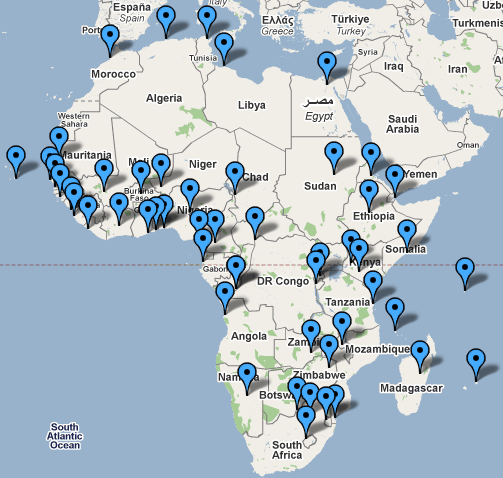
\includegraphics[scale=0.60]{points.png}}
    \caption{Capitals of African Nations}
  \end{center}
\end{figure}


\begin{multicols}{3}
\tiny\begin{enumerate*}
\item Algeria - Algiers
\item Angola - Luanda
\item Benin - Porto-Novo
\item Botswana - Gaborone
\item Burkina Faso - Ouagadougou
\item Burundi - Bujumbura
\item Cameroon - Yaounde
\item Cape Verde - Praia
\item Central African Republic - Bangui
\item Chad - N'Djamena
\item Comoros - Moroni
\item Congo, Republic of the - Brazzaville
\item Congo, Democratic Republic of the - Kinshasa
\item Cote d'Ivoire - Yamoussoukro
\item Djibouti - Djibouti
\item Egypt - Cairo
\item Equatorial Guinea - Malabo
\item Eritrea - Asmara
\item Ethiopia - Addis Ababa
\item Gabon - Libreville
\item The Gambia - Banjul
\item Ghana - Accra
\item Guinea - Conakry
\item Guinea-Bissau - Bissau
\item Kenya - Nairobi
\item Lesotho - Maseru
\item Liberia - Monrovia
\item Libya - Tripoli
\item Madagascar - Antananarivo
\item Malawi - Lilongwe
\item Mali - Bamako
\item Mauritania - Nouakchott
\item Mauritius - Port Louis
\item Morocco - Rabat
\item Mozambique - Maputo
\item Namibia - Windhoek
\item Niger - Niamey
\item Nigeria - Abuja
\item Rwanda - Kigali
\item Senegal - Dakar
\item Seychelles - Victoria
\item Sierra Leone - Freetown
\item Somalia - Mogadishu
\item South Africa - Pretoria
\item Sudan - Khartoum
\item Swaziland - Mbabane
\item Tanzania - Dar es Salaam
\item Togo - Lome
\item Tunisia - Tunis
\item Uganda - Kampala
\item Zambia - Lusaka
\item Zimbabwe - Harare
\end{enumerate*}
\end{multicols}

\section{Overview}

  The traveling salesman problem (TSP) is a thoroughly researched problem in theoretically computer-science. 
TSP is classified as NP-Hard e.g. it is as hard or harder to solve than a problem solvable in nondeterministic polynomial time.
This means the worst case performance for a TSP algorithm will likely increase exponentially with the numbers of cities to traverse.
The big-O complexity of a brute force TSP algorithms (check all vertices against all other vertices) is $O(n!)$.

  I attempted to solve the TSP with both a brute force method initially and eventually a simulated annealing algorithm. 
Both implementation's rely on the pythong programming language and it's random number implementation to generate new routes.
The brute force algorithm simply attempts all combinations, giving priority to each new best performing route.
This algorithm performed well, yielding great result's, but I felt it would be beneficial to try another approach. 
Simulated annealing is often cited as a relatively easy way to improve TSP performance.

\begin{quotation}\bf``\normalfont Simulated annealing starts with the cities connected in a random order, and then considers making random changes in that order. If changing the order of cities leads to a shorter path, we accept that change. If the modification yields a longer path, we give ourselves a certain probability of accepting the modification -- less likely the larger the proposed increase in path length. We then gradually reduce this probability over time, in order to rule out shorter and shorter path increases -- thereby converging toward a path length close to the absolute minimum.\bf''\normalfont\cite{sa} \end{quotation}
\section{Programs}

\begin{enumerate}
\item The Python 2.6 \cite{python} programming language and interpreter.
\item Wikipedia provides a convenient list of latitude/longitude pairs for all major cities in the world. This was cross referenced with
the list of African nations and capitals recognized by the United Nations.\cite{wiki}
\item Software originally written by John Montgomery \cite{tsp} in 2007. It was a general exercise in implementing different types of TSP algorithms. At this point it's been heavily modified to meet my needs for this project.
\item The results were then visualized using Google maps static mapping API. \cite{google}
\item A general algorithm for computing the distance between two latitude/longitude points.\cite{dis}
\end{enumerate}


\section{Solution}

%$yDis = ( lat2 - lat1 ) * \text{Nautical Miles Per Latitude}$\newline
%$xDis = ( \cos( lat1 - \frac{\pi}{180} ) + \cos( lat2 - \frac{\pi}{180} ) ) * ( lon2 - lon1 ) * \frac{\text{Nautical Miles Per Longitude}}{2}$\newline
%$tDistance = \sqrt{ yDis^{2} + xDis^{2} } * \text{Miles per Nautical Miles}$\newline

\begin{figure}[!h]
  \begin{center}
    \setlength\fboxsep{1.00pt}
    \setlength\fboxrule{1.00pt}
    \fbox{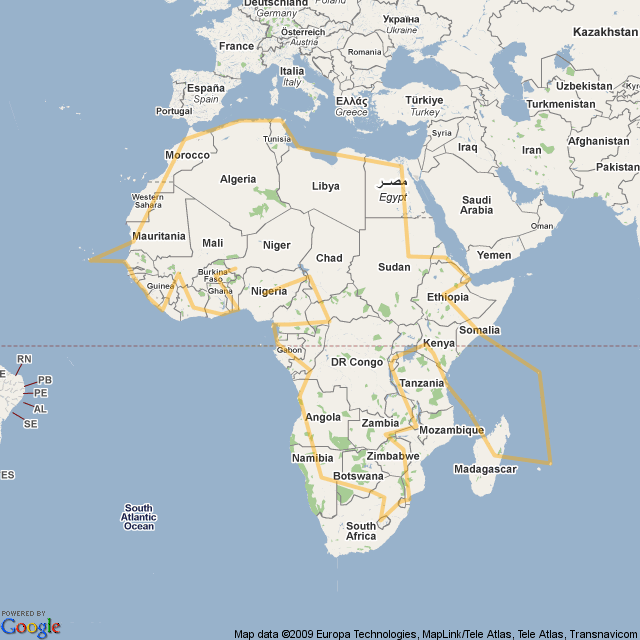
\includegraphics[scale=0.50]{path.png}}
    \caption{Final Round Trip Path Through Africa}
  \end{center}
\end{figure}

Final Round Trip Order:
\begin{multicols}{3}
\tiny\begin{enumerate*}
\item Congo, Republic of the - Brazzaville
\item Congo, Democratic Republic of the - Kinshasa
\item Angola - Luanda
\item Namibia - Windhoek
\item Botswana - Gaborone
\item South Africa - Pretoria
\item Lesotho - Maseru
\item Swaziland - Mbabane
\item Mozambique - Maputo
\item Zimbabwe - Harare
\item Zambia - Lusaka
\item Malawi - Lilongwe
\item Burundi - Bujumbura
\item Rwanda - Kigali
\item Uganda - Kampala
\item Kenya - Nairobi
\item Tanzania - Dar es Salaam
\item Comoros - Moroni
\item Madagascar - Antananarivo
\item Mauritius - Port Louis
\item Seychelles - Victoria
\item Somalia - Mogadishu
\item Ethiopia - Addis Ababa
\item Djibouti - Djibouti
\item Eritrea - Asmara
\item Sudan - Khartoum
\item Egypt - Cairo
\item Libya - Tripoli
\item Tunisia - Tunis
\item Algeria - Algiers
\item Morocco - Rabat
\item Mauritania - Nouakchott
\item Cape Verde - Praia
\item Senegal - Dakar
\item The Gambia - Banjul
\item Guinea-Bissau - Bissau
\item Guinea - Conakry
\item Sierra Leone - Freetown
\item Liberia - Monrovia
\item Cote d'Ivoire - Yamoussoukro
\item Mali - Bamako
\item Burkina Faso - Ouagadougou
\item Niger - Niamey
\item Ghana - Accra
\item Togo - Lome
\item Benin - Porto-Novo
\item Nigeria - Abuja
\item Chad - N'Djamena
\item Central African Republic - Bangui
\item Cameroon - Yaounde
\item Equatorial Guinea - Malabo
\item Gabon - Libreville
\end{enumerate*}
\end{multicols}

Total Length Of Round Trip Route $\approx 35,813 km$ \newline

Route Without Round Trip Stipulation:
\begin{multicols}{3}
\tiny\begin{enumerate*}
\item Benin - Porto-Novo
\item Togo - Lome
\item Ghana - Accra
\item Niger - Niamey
\item Burkina Faso - Ouagadougou
\item Mali - Bamako
\item Cote d'Ivoire - Yamoussoukro
\item Liberia - Monrovia
\item Sierra Leone - Freetown
\item Guinea - Conakry
\item Guinea-Bissau - Bissau
\item The Gambia - Banjul
\item Senegal - Dakar
\item Mauritania - Nouakchott
\item Cape Verde - Praia
\item Morocco - Rabat
\item Algeria - Algiers
\item Tunisia - Tunis
\item Libya - Tripoli
\item Egypt - Cairo
\item Sudan - Khartoum
\item Eritrea - Asmara
\item Djibouti - Djibouti
\item Ethiopia - Addis Ababa
\item Somalia - Mogadishu
\item Seychelles - Victoria
\item Mauritius - Port Louis
\item Madagascar - Antananarivo
\item Comoros - Moroni
\item Tanzania - Dar es Salaam
\item Kenya - Nairobi
\item Uganda - Kampala
\item Rwanda - Kigali
\item Burundi - Bujumbura
\item Malawi - Lilongwe
\item Zambia - Lusaka
\item Zimbabwe - Harare
\item Mozambique - Maputo
\item Swaziland - Mbabane
\item Lesotho - Maseru
\item South Africa - Pretoria 
\item Botswana - Gaborone
\item Namibia - Windhoek
\item Angola - Luanda
\item Congo, Democratic Republic of the - Kinshasa
\item Congo, Republic of the - Brazzaville
\item Central African Republic - Bangui
\item Chad - N'Djamena
\item Cameroon - Yaounde
\item Gabon - Libreville
\item Equatorial Guinea - Malabo
\item Nigeria - Abuja
\end{enumerate*}
\end{multicols}

Total Length Of Non-Round-trip Route $\approx 34,096 km$

\section{Runtime}

The two algorithms, simulated annealing and brute force random permutations where both run in numerous instances over the life of the project. 
In combined total they were run upwards of fifty times a piece.

The version of the algorithm which used simulated annealing on average found the optimal solution in approximately 6 seconds. 
While the brute force algorithm delivered the same result or close to it in upwards of 2 to 10 minutes. Given the internal implementation of the algorithm, it's performance is directly linked with the first random number used to seed the initial route.
Multiple runs of the brute force algorithm another one another often result in drastically different run times to find the same solution. This was beyond my control on the implementation side of things.

\section{Analysis}

I believe the final optimal path's are within a reasonable uncertainty of the actual path.
Given the big-O of the brute force algorithm, $O(n!)$ or $O( 8.065 \times 10^{67} )$, a runtime complexity of this magnitude is obviously out of my league for finding exact values.
At a maximum I was able to attempt 100,000,000 permutations of the path.

Two area's of possible improvement I can pinpoint are:
\begin{enumerate}
\item The language itself. I chose the python programming language for my TSP implementation.
The language is interpreted and it's runtime speed can at times be 20\% slower than an equivalent C program.
\item The random.shuffle implementation. Given how python's random.shuffle API is implemented it takes a set
of values and shuffles them based on a random number between 0,1 generated by the operating system. However given the size of the set
, 52 individual points, the likely hood that random.shuffle will generated all permutations without excessive doubles is incredibly unlikely.
This is the cause of a lot of useless computation time, however because of the size of the data set, caching data sets is not plausible let alone if even possible.
\end{enumerate}

Re-writing the algorithm in C would be a great performance benefit. Also having a proper resources to cache routes or a effective random route generator I believe a more accurate optimal route might be found.

It is also worth mentioning that after completing a large part of the project I discovered the LHK\cite{LHK} high performance TSP solver. It's written in straight C and requires the dataset to be in a very specific format.
Given more time to organize the dataset into the proper format, I believe the LHK solver might produce a more accurate route given a much larger number of iterations. 
\begin{thebibliography}{99}
\bibitem{python} {\href{ http://python.org }{ http://python.org }}
\bibitem{wiki} {\href{ http://en.wikipedia.org/wiki/Latitude_and_longitude_of_cities }{ http://en.wikipedia.org/wiki/Latitude\_and\_longitude\_of\_cities }}
\bibitem{tsp} Montgomery, John {\it Tackling The Travelling Salesman Problem }{\href{ http://www.psychicorigami.com/category/tsp/ }{ http://www.psychicorigami.com/category/tsp/ } }, {\bf 2007}
\bibitem{google} {\href{ http://code.google.com/apis/maps/documentation/staticmaps/  }{ http://code.google.com/apis/maps/documentation/staticmaps/ }}
\bibitem{sa}{\href{ http://www.svengato.com/salesman.html }{ http://www.svengato.com/salesman.html }}
\bibitem{dis}{\href{ http://www.geesblog.com/2009/01/calculating-distance-between-latitude-longitude-pairs-in-python/ }{ http://www.geesblog.com/2009/01/calculating-distance-between-latitude-longitude-pairs-in-python/ }}
\bibitem{LHK}{\href{ http://www.akira.ruc.dk/~keld/research/LKH/ }{ http://www.akira.ruc.dk/~keld/research/LKH/ }}

\end{thebibliography}
\section{Program Output}
\tiny\begin{verbatim}
burny ~/src/traveling-salesman $ python tsp.py -v -a anneal -n 1000000 --cooling 10:.9991 ../latlon
2009-11-02 00:43:38,822 INFO using move_operator: <function reversed_sections at 0x745f0>
2009-11-02 00:43:38,860 INFO new best score: -111551.944723
2009-11-02 00:43:38,861 INFO anneal started: score=-111551.944723
2009-11-02 00:43:38,861 INFO current run at 2 runs
2009-11-02 00:43:38,861 INFO current run at 4 runs
2009-11-02 00:43:38,861 INFO new best score: -108938.423206
2009-11-02 00:43:38,862 INFO new best score: -108255.962603
2009-11-02 00:43:38,862 INFO current run at 8 runs
2009-11-02 00:43:38,862 INFO new best score: -107174.578311
2009-11-02 00:43:38,862 INFO new best score: -107174.578311
2009-11-02 00:43:38,862 INFO new best score: -106843.737327
2009-11-02 00:43:38,863 INFO current run at 16 runs
2009-11-02 00:43:38,864 INFO new best score: -105825.989448
2009-11-02 00:43:38,864 INFO new best score: -105805.630085
2009-11-02 00:43:38,864 INFO new best score: -105428.930412
2009-11-02 00:43:38,864 INFO new best score: -103871.898541
2009-11-02 00:43:38,865 INFO new best score: -99956.329397
2009-11-02 00:43:38,865 INFO current run at 32 runs
2009-11-02 00:43:38,865 INFO new best score: -99252.982749
2009-11-02 00:43:38,865 INFO new best score: -96688.656537
2009-11-02 00:43:38,866 INFO new best score: -94637.985111
2009-11-02 00:43:38,866 INFO new best score: -92809.021849
2009-11-02 00:43:38,866 INFO new best score: -92567.648622
2009-11-02 00:43:38,867 INFO new best score: -92341.764572
2009-11-02 00:43:38,867 INFO new best score: -92019.656620
2009-11-02 00:43:38,867 INFO new best score: -91759.417996
2009-11-02 00:43:38,867 INFO new best score: -91657.533796
2009-11-02 00:43:38,867 INFO new best score: -91615.252931
2009-11-02 00:43:38,868 INFO new best score: -91510.009964
2009-11-02 00:43:38,868 INFO new best score: -91409.900530
2009-11-02 00:43:38,868 INFO new best score: -88486.992310
2009-11-02 00:43:38,869 INFO new best score: -87865.530081
2009-11-02 00:43:38,869 INFO current run at 64 runs
2009-11-02 00:43:38,870 INFO new best score: -84271.022595
2009-11-02 00:43:38,871 INFO new best score: -83806.794411
2009-11-02 00:43:38,871 INFO new best score: -83541.482139
2009-11-02 00:43:38,873 INFO new best score: -83230.783927
2009-11-02 00:43:38,873 INFO new best score: -82737.304308
2009-11-02 00:43:38,874 INFO new best score: -81484.288842
2009-11-02 00:43:38,874 INFO new best score: -78113.454255
2009-11-02 00:43:38,875 INFO new best score: -78076.761685
2009-11-02 00:43:38,876 INFO current run at 128 runs
2009-11-02 00:43:38,876 INFO new best score: -77590.182221
2009-11-02 00:43:38,876 INFO new best score: -77048.097861
2009-11-02 00:43:38,876 INFO new best score: -75684.545805
2009-11-02 00:43:38,877 INFO new best score: -75404.373749
2009-11-02 00:43:38,877 INFO new best score: -75171.746424
2009-11-02 00:43:38,878 INFO new best score: -74321.762810
2009-11-02 00:43:38,879 INFO new best score: -73252.833808
2009-11-02 00:43:38,879 INFO new best score: -73104.514189
2009-11-02 00:43:38,881 INFO new best score: -72788.614518
2009-11-02 00:43:38,881 INFO new best score: -72591.656921
2009-11-02 00:43:38,881 INFO new best score: -70578.358239
2009-11-02 00:43:38,882 INFO new best score: -68799.506394
2009-11-02 00:43:38,883 INFO new best score: -68619.887877
2009-11-02 00:43:38,884 INFO new best score: -67121.606526
2009-11-02 00:43:38,884 INFO new best score: -66626.493200
2009-11-02 00:43:38,884 INFO new best score: -64344.816135
2009-11-02 00:43:38,884 INFO new best score: -64230.900991
2009-11-02 00:43:38,885 INFO new best score: -64101.038316
2009-11-02 00:43:38,885 INFO new best score: -63926.594272
2009-11-02 00:43:38,886 INFO new best score: -63639.151393
2009-11-02 00:43:38,886 INFO new best score: -63342.571435
2009-11-02 00:43:38,886 INFO new best score: -62883.123482
2009-11-02 00:43:38,886 INFO new best score: -60493.251630
2009-11-02 00:43:38,887 INFO new best score: -58493.381705
2009-11-02 00:43:38,888 INFO new best score: -58364.904831
2009-11-02 00:43:38,888 INFO new best score: -57861.729512
2009-11-02 00:43:38,889 INFO new best score: -57785.659587
2009-11-02 00:43:38,889 INFO new best score: -56237.272807
2009-11-02 00:43:38,889 INFO current run at 256 runs
2009-11-02 00:43:38,890 INFO new best score: -52752.018487
2009-11-02 00:43:38,890 INFO new best score: -52058.361255
2009-11-02 00:43:38,890 INFO new best score: -51827.173423
2009-11-02 00:43:38,891 INFO new best score: -50650.559834
2009-11-02 00:43:38,894 INFO new best score: -50540.078096
2009-11-02 00:43:38,895 INFO new best score: -50317.193191
2009-11-02 00:43:38,895 INFO new best score: -48975.975547
2009-11-02 00:43:38,896 INFO new best score: -48849.972600
2009-11-02 00:43:38,898 INFO new best score: -48838.291771
2009-11-02 00:43:38,902 INFO new best score: -48368.567964
2009-11-02 00:43:38,903 INFO new best score: -46559.324605
2009-11-02 00:43:38,904 INFO new best score: -46558.360448
2009-11-02 00:43:38,905 INFO new best score: -46522.611077
2009-11-02 00:43:38,905 INFO new best score: -46422.331395
2009-11-02 00:43:38,906 INFO new best score: -44981.634651
2009-11-02 00:43:38,907 INFO new best score: -44820.384544
2009-11-02 00:43:38,907 INFO new best score: -44643.673209
2009-11-02 00:43:38,909 INFO new best score: -44004.657313
2009-11-02 00:43:38,909 INFO new best score: -43563.669128
2009-11-02 00:43:38,910 INFO new best score: -43510.757103
2009-11-02 00:43:38,912 INFO current run at 512 runs
2009-11-02 00:43:38,916 INFO new best score: -42977.735342
2009-11-02 00:43:38,916 INFO new best score: -41456.278999
2009-11-02 00:43:38,917 INFO new best score: -41383.345365
2009-11-02 00:43:38,918 INFO new best score: -40087.086741
2009-11-02 00:43:38,919 INFO new best score: -39434.670603
2009-11-02 00:43:38,919 INFO new best score: -39219.990542
2009-11-02 00:43:38,921 INFO new best score: -38293.656546
2009-11-02 00:43:38,924 INFO new best score: -36738.445888
2009-11-02 00:43:38,926 INFO new best score: -36649.112566
2009-11-02 00:43:38,932 INFO new best score: -36591.647201
2009-11-02 00:43:38,933 INFO new best score: -36238.421358
2009-11-02 00:43:38,935 INFO new best score: -36196.494534
2009-11-02 00:43:38,938 INFO new best score: -36014.634524
2009-11-02 00:43:38,940 INFO new best score: -35991.037879
2009-11-02 00:43:38,941 INFO new best score: -35889.038030
2009-11-02 00:43:38,946 INFO new best score: -35667.660601
2009-11-02 00:43:38,953 INFO new best score: -35491.868203
2009-11-02 00:43:38,955 INFO current run at 1024 runs
2009-11-02 00:43:38,958 INFO new best score: -35322.422385
2009-11-02 00:43:38,971 INFO new best score: -35296.389295
2009-11-02 00:43:38,972 INFO new best score: -34799.198370
2009-11-02 00:43:38,974 INFO new best score: -34655.194786
2009-11-02 00:43:38,977 INFO new best score: -34608.069227
2009-11-02 00:43:38,979 INFO new best score: -34539.947513
2009-11-02 00:43:38,979 INFO new best score: -33247.031299
2009-11-02 00:43:38,979 INFO new best score: -32367.878943
2009-11-02 00:43:38,987 INFO new best score: -31805.170969
2009-11-02 00:43:38,996 INFO new best score: -31465.390351
2009-11-02 00:43:38,996 INFO new best score: -31399.347724
2009-11-02 00:43:38,999 INFO new best score: -30749.273747
2009-11-02 00:43:39,003 INFO new best score: -30425.747441
2009-11-02 00:43:39,005 INFO new best score: -29257.455498
2009-11-02 00:43:39,006 INFO new best score: -29215.783892
2009-11-02 00:43:39,008 INFO new best score: -28975.291472
2009-11-02 00:43:39,012 INFO new best score: -28192.624760
2009-11-02 00:43:39,018 INFO new best score: -27934.421265
2009-11-02 00:43:39,026 INFO new best score: -27688.247659
2009-11-02 00:43:39,035 INFO current run at 2048 runs
2009-11-02 00:43:39,037 INFO new best score: -27390.644387
2009-11-02 00:43:39,057 INFO new best score: -26793.922438
2009-11-02 00:43:39,057 INFO new best score: -26696.244150
2009-11-02 00:43:39,061 INFO new best score: -26404.136400
2009-11-02 00:43:39,083 INFO new best score: -26404.136400
2009-11-02 00:43:39,094 INFO new best score: -25926.038197
2009-11-02 00:43:39,108 INFO new best score: -25368.028231
2009-11-02 00:43:39,115 INFO new best score: -25312.586966
2009-11-02 00:43:39,132 INFO new best score: -25251.911826
2009-11-02 00:43:39,137 INFO new best score: -25202.999277
2009-11-02 00:43:39,145 INFO new best score: -24692.239918
2009-11-02 00:43:39,158 INFO new best score: -24692.239918
2009-11-02 00:43:39,187 INFO new best score: -24206.877575
2009-11-02 00:43:39,195 INFO current run at 4096 runs
2009-11-02 00:43:39,223 INFO new best score: -24159.595396
2009-11-02 00:43:39,231 INFO new best score: -24088.719891
2009-11-02 00:43:39,245 INFO new best score: -23972.734353
2009-11-02 00:43:39,260 INFO new best score: -23906.426074
2009-11-02 00:43:39,289 INFO new best score: -23901.325907
2009-11-02 00:43:39,305 INFO new best score: -23286.130255
2009-11-02 00:43:39,309 INFO new best score: -23076.669258
2009-11-02 00:43:39,310 INFO new best score: -22945.476729
2009-11-02 00:43:39,320 INFO new best score: -22943.882305
2009-11-02 00:43:39,370 INFO new best score: -22097.219253
2009-11-02 00:43:39,378 INFO new best score: -21951.069041
2009-11-02 00:43:39,512 INFO current run at 8192 runs
2009-11-02 00:43:39,769 INFO new best score: -21949.474618
2009-11-02 00:43:40,134 INFO current run at 16384 runs
2009-11-02 00:43:40,367 INFO new best score: -21819.103878
2009-11-02 00:43:40,368 INFO new best score: -21814.003710
2009-11-02 00:43:40,430 INFO new best score: -21812.409286
2009-11-02 00:43:40,442 INFO new best score: -21812.409286
2009-11-02 00:43:41,231 INFO new best score: -21729.582347
2009-11-02 00:43:41,262 INFO new best score: -21604.015041
2009-11-02 00:43:42,573 INFO new best score: -21549.955257
2009-11-02 00:43:43,565 INFO current run at 32768 runs
2009-11-02 00:43:43,652 INFO new best score: -21549.955257
2009-11-02 00:43:45,122 INFO new best score: -21549.955257
2009-11-02 00:43:48,326 INFO current run at 65536 runs
2009-11-02 00:43:54,024 INFO current run at 131072 runs
2009-11-02 00:44:05,620 INFO current run at 262144 runs
2009-11-02 00:44:29,461 INFO current run at 524288 runs
2009-11-02 00:45:13,352 INFO final temperature: 1.232621
2009-11-02 00:45:13,352 INFO anneal finished: num_evaluations=1000000, best_score=-21549.955257
Benin - Porto-Novo
Togo - Lome
Ghana - Accra
Niger - Niamey
Burkina Faso - Ouagadougou
Cote d'Ivoire - Yamoussoukro
Liberia - Monrovia
Sierra Leone - Freetown
Guinea - Conakry
Guinea-Bissau - Bissau
The Gambia - Banjul
Senegal - Dakar
Mauritania - Nouakchott
Cape Verde - Praia
Morocco - Rabat
Algeria - Algiers
Tunisia - Tunis
Libya - Tripoli
Egypt - Cairo
Sudan - Khartoum
Eritrea - Asmara
Djibouti - Djibouti
Ethiopia - Addis Ababa
Somalia - Mogadishu
Seychelles - Victoria
Mauritius - Port Louis
Madagascar - Antananarivo
Comoros - Moroni
Tanzania - Dar es Salaam
Kenya - Nairobi
Uganda - Kampala
Rwanda - Kigali
Burundi - Bujumbura
Malawi - Lilongwe
Zambia - Lusaka
Zimbabwe - Harare
Mozambique - Maputo
Swaziland - Mbabane
Lesotho - Maseru
South Africa - Pretoria 
Botswana - Gaborone
Namibia - Windhoek
Angola - Luanda
Congo, Democratic Republic of the - Kinshasa
Congo, Republic of the - Brazzaville
Central African Republic - Bangui
Chad - N'Djamena
Cameroon - Yaounde
Gabon - Libreville
Equatorial Guinea - Malabo
Nigeria - Abuja
21186.3444977 mi
\end{verbatim}

\end{document}
